% eLife derivative manuscript template
%%% PREAMBLE 
\documentclass[9pt]{elife}

\usepackage{bm}
\usepackage{caption}
\usepackage{float}
\usepackage{listings}
\usepackage{multirow}
\usepackage{siunitx}
\usepackage{subcaption}
\usepackage{soul}
\usepackage{adjustbox}
\usepackage{hyperref}
\usepackage{academicons}
\usepackage{xcolor}
\newcommand{\orcid}[1]{\href{https://orcid.org/#1}{\textcolor{HTML}{A6CE39}{\aiOrcid}}}

\graphicspath{ {./Figures/} }

\setlength{\marginparwidth}{2cm}

%%%%%%%%%%%%%%%%%%%%%%%%%%%%%%%%%%%%%%%%%%%%%%%%%%%%%%%%%%%%
%%% ARTICLE SETUP
%%%%%%%%%%%%%%%%%%%%%%%%%%%%%%%%%%%%%%%%%%%%%%%%%%%%%%%%%%%%
\title{\huge Supporting Information: Identifying signatures of proteolytic stability and monomeric propensity in \emph{O}-glycosylated insulin using molecular simulation}

\author[1]{Wei-Tse Hsu}
\author[2]{Dominique A. Ramirez}
\author[3]{Tarek Sammakia}
\author[4]{Zhongping Tan}
\author[1]{Michael R. Shirts}

\affil[1]{Department of Chemical \& Biological Engineering, University of Colorado Boulder, Boulder, CO, USA 80309}
\affil[2]{Department of Biochemistry, University of Colorado Boulder, Boulder, CO, USA 80309}
\affil[3]{Department of Chemistry, University of Colorado Boulder, Boulder, CO, USA 80309}
\affil[4]{Institute of Materia Medica, Chinese Academy of Medical Sciences, Peking Union Medical College, Beijing, 100050, China}

\corr{michael.shirts@colorado.edu}{MRS}
\corr{zhongping.tan@imm.pumc.edu.cn}{ZT}

\contrib{\small Submitted in the Journal of Computer-Aided Molecular Design.}

%%%%%%%%%%%%%%%%%%%%%%%%%%%%%%%%%%%%%%%%%%%%%%%%%%%%%%%%%%%%
%%% ARTICLE START
%%%%%%%%%%%%%%%%%%%%%%%%%%%%%%%%%%%%%%%%%%%%%%%%%%%%%%%%%%%%

\begin{document}

\maketitle

%===============================
% Supporting Information
%===============================
\section{Supplemental Tables}

\renewcommand{\thetable}{S\arabic{table}}
\begin{table}[H]
\centering
\begin{tabular}{|c|c|c|c|c|c|}

\hline
     & 4EYD & 4EY1 & 3I3Z & 4EY9 & 2MVC \\
\hline
Total charges & -1 & -1 & -1 & -1 & -1 \\
\hline
pH value & 8.0 & 8.0 & 7.9 & 6.9 & 7.3 \\
\hline
HisB5 & HIP (+1) &HIP (+1) &HIP (+1) &HIP (+1) & HIE (+0) \\
\hline
HisB10 & HIE (+0) & HIE (+0) &HIE (+0) &HID (+0) & HIP (+1)  \\
\hline
\end{tabular}
\caption{The comparison of histidine protonation states of wild-type structures.}
\label{supple_tab: protonation}
\end{table}

\renewcommand{\thetable}{S\arabic{table}}
\begin{table}[H]
\centering
\begin{adjustbox}{width=1.0\textwidth,center=\textwidth}
\begin{tabular}{|l| c| c| c| c| c| c| c| c| c| c| c| c|}
\hline
&GF 2&GF 3&GF 4&GF 5&GF 6&GF 7&GF 8&GF 9&GF 10&GF 11&GF 12&GF 13\\ \hline
4EYD&NA& NA&3.45&63.56&69.11& NA& NA&45.79&121.70&21.65&140.40&24.77 \\ \hline
4EY1&NA& NA&6.89&371.83&71.04& NA&19.37&205.24&159.14&58.17&360.45&637.20 \\ \hline
4EY9&NA & NA &18.53&274.66&97.34& NA &NA &12.55&496.98&0.39&89.13&57.77 \\ \hline
3I3Z&NA & NA &93.49&62.86&199.65& NA & NA &45.27&62.80&42.78&97.81&281.52 \\ \hline
2MVC&3.98&NA &21.31&54.78&105.28&NA &NA &114.61&59.62&58.75&66.00&81.57 \\ \hline
\end{tabular}
\end{adjustbox}
\caption{Dimer occlusion autocorrelation lag times for each of the listed models. All numbers are listed in units of nanoseconds.}
\label{supple_tab: occlusion_lag}
\end{table}

\begin{table}[H]
\begin{adjustbox}{width=1\textwidth}
\begin{tabular}{|c|c|c|c|c|c|}
\hline
\# & 4EYD-based GFs                                                                                                                             & 4EY1-based GFs                                                                                                                                                             & 4EY9-based GFs                                                                                                                                                             & 3I3Z-based GFs                                                                                                                            & 2MVC-based GFs                                                                                                                            \\ \hline
1  & N/A                                                                                                                                        & N/A                                                                                                                                                                        & N/A                                                                                                                                                                        & N/A                                                                                                                                       & N/A                                                                                                                                       \\ \hline
2  & None                                                                                                                                       & ThrA8(OG1)-GalNAc{[}1{]}(O2N):10\%                                                                                                                                         & None                                                                                                                                                                       & None                                                                                                                                      & \begin{tabular}[c]{@{}c@{}}GlnA5(NE2)-GalNAc{[}1{]}(O6): 14\%\\ GlnA15(NE2)-GalNAc{[}1{]}(O6): 13\%\end{tabular}                          \\ \hline
3  & None                                                                                                                                       & None                                                                                                                                                                       & None                                                                                                                                                                       & None                                                                                                                                      & GlnA15(NE2)-52(O2N):11\%                                                                                                                  \\ \hline
4  & None                                                                                                                                       & None                                                                                                                                                                       & None                                                                                                                                                                       & None                                                                                                                                      & None                                                                                                                                      \\ \hline
5  & None                                                                                                                                       & \begin{tabular}[c]{@{}c@{}}PheB24(N)-GalNAc{[}1{]}(O3): 48\%\\ ThrB30(N)-GalNAc{[}1{]}(O2N): 16\%\end{tabular}                                                             & PheB24(N)-GalNAc{[}1{]}(O3): 11\%                                                                                                                                          & \begin{tabular}[c]{@{}c@{}}ThrB27(N)-GalNAc{[}1{]}(O3):15\%\\ Glu4(N)-GalNAc{[}1{]}(O2N): 14\%\end{tabular}                               & PheB24(N)-GalNAc{[}1{]}(O3): 10\%                                                                                                         \\ \hline
6  & ThrB27(N)-GalNAc{[}1{]}(O3):26\%                                                                                                           & ThrB27(N)-GalNAc(1)(O3):26\%                                                                                                                                               & None                                                                                                                                                                       & None                                                                                                                                      & \begin{tabular}[c]{@{}c@{}}CysA7(N)-GalNAc{[}1{]}(O2N): 18\%\\ ThrB27(N)-GalNAc(1)(O3): 12\%\end{tabular}                                 \\ \hline
7  & None                                                                                                                                       & None                                                                                                                                                                       & None                                                                                                                                                                       & None                                                                                                                                      & GlnA15(NE2)-Man{[}1{]}(O4): 18\%                                                                                                          \\ \hline
8  & GlnA5(NE2)-Man{[}2{]}(O2): 12\%                                                                                                            & GlnA5(NE2)-Man{[}2{]}(O2): 11\%                                                                                                                                            & None                                                                                                                                                                       & GlnA5(NE2)-Man{[}1{]}(O5): 12\%                                                                                                           & None                                                                                                                                      \\ \hline
9  & \begin{tabular}[c]{@{}c@{}}PheB24(N)-Man{[}1{]}(O3): 22\%\\ TyrB16(OH)-Man{[}1{]}(O4): 13\%\end{tabular}                                   & None                                                                                                                                                                       & \begin{tabular}[c]{@{}c@{}}PheB24(N)-Man{[}1{]}(O3): 27\%\\ TyrB16(OH)-Man{[}1{]}(O4): 19\%\end{tabular}                                                                   & None                                                                                                                                      & None                                                                                                                                      \\ \hline
10 & \begin{tabular}[c]{@{}c@{}}PheB24(N)-Man{[}1{]}(O3): 52\%\\ ThrB30(N)--Man{[}2{]}(O2): 35\%\\ ThrB27(N)--Man{[}2{]}(O6): 23\%\end{tabular} & \begin{tabular}[c]{@{}c@{}}ThrB27(N)-Man{[}2{]}(O6): 46\%\\ PheB24(N)-Man{[}1{]}(O3): 30\%\\ TyrB16(OH)-Man{[}1{]}(O4): 15\%\end{tabular}                                  & \begin{tabular}[c]{@{}c@{}}ThrB27(N)-Man{[}2{]}(O6): 45\%\\ PheB24(N)-Man{[}1{]}(O3): 28\%\\ TyrB16(OH)-Man{[}1{]}(O4): 11\%\end{tabular}                                  & \begin{tabular}[c]{@{}c@{}}ThrB27(N)-Man{[}2{]}(O6): 47\%\\ PheB24(N)-Man{[}1{]}(O3): 15\%\end{tabular}                                   & \begin{tabular}[c]{@{}c@{}}ThrB27(N)-Man{[}2{]}(O6): 47\%\\ PheB24(N)-Man{[}1{]}(O3): 37\%\\ TyrB16(OH)-Man{[}1{]}(O4): 14\%\end{tabular} \\ \hline
11 & None                                                                                                                                       & None                                                                                                                                                                       & None                                                                                                                                                                       & None                                                                                                                                      & None                                                                                                                                      \\ \hline
12 & \begin{tabular}[c]{@{}c@{}}ThrB30(N)-Man{[}2{]}(O6): 31\%\\ GlyB23(N)-Man{[}1{]}(O3): 10\%\end{tabular}                                    & \begin{tabular}[c]{@{}c@{}}TyrA19(OH)-Man{[}1{]}(O4): 51\%\\ ThrB27(N)-Man{[}1{]}(O3): 43\%\\ ThrB30(N)-Man{[}2{]}(O6): 19\%\end{tabular}                                  & \begin{tabular}[c]{@{}c@{}}ThrB30(N)-Man{[}2{]}(O6): 24\%\\ ValA3(N)-Man{[}2{]}(O2): 15\%\end{tabular}                                                                     & ThrB30(N)--Man{[}2{]}(O6): 38\%                                                                                                           & \begin{tabular}[c]{@{}c@{}}ThrB30(N)-Man{[}2{]}(O6): 49\%\\ GlyB8(N)-Man{[}2{]}(O4): 10\%\end{tabular}                                    \\ \hline
13 & \begin{tabular}[c]{@{}c@{}}ThrB27(N)-Man{[}2{]}(O6): 61\%\\ PheB24(N)-Man{[}1{]}(O3): 49\%\\ TyrB16(OH)-Man{[}1{]}(O4): 16\%\end{tabular}  & \begin{tabular}[c]{@{}c@{}}ThrB27(N)-Man{[}2{]}(O6): 31\%\\ ThrB27(N)-Man{[}3{]}(O6): 14\%\\ PheB24(N)-Man{[}1{]}(O3): 12\%\\ TyrB16(OH)-Man{[}1{]}(O4): 11\%\end{tabular} & \begin{tabular}[c]{@{}c@{}}ThrB27(N)-Man{[}2{]}(O6): 27\%\\ PheB24(N)-Man{[}1{]}(O3): 17\%\\ ThrB27(N)-Man{[}3{]}(O6): 15\%\\ TyrB16(OH)-Man{[}1{]}(O4): 10\%\end{tabular} & \begin{tabular}[c]{@{}c@{}}ThrB27(N)-Man{[}2{]}(O6): 43\%\\ PheB24(N)-Man{[}1{]}(O3): 25\%\\ TyrB16(OH)-Man{[}1{]}(O4): 12\%\end{tabular} & \begin{tabular}[c]{@{}c@{}}ThrB27(N)-Man{[}2{]}(O6): 44\%\\ PheB24(N)-Man{[}1{]}(O3): 22\%\end{tabular}                                   \\ \hline
\end{tabular}
\end{adjustbox}
\caption{The glycan-involved hydrogen bonds and their existence percentages of each glycoform.}
\label{supple_tab: hbond}
\end{table}

% atom type table
\begin{table}[H]
\centering
\begin{tabular}{|c|c|c|}
\hline
Atom type & Role     & Description                                                      \\ \hline
N         & Donor    & An sp$^{2}$ nitrogen in amide group                              \\ \hline
NE2       & Donor    & An epsilon nitrogen.                                             \\ \hline
OH        & Donor    & An alcohol oxygen in Tyr                                        \\ \hline
OG1       & Donor    & An alcohol oxygen in Thr                                        \\ \hline
O2        & Acceptor & The oxygen atom connected to the second carbon atom of the sugar \\ \hline
O3        & Acceptor & The oxygen atom connected to the third carbon atom of the sugar  \\ \hline
O4        & Acceptor & The oxygen atom connected to the fourth carbon atom of the sugar \\ \hline
O5        & Acceptor & The oxygen atom connected to the fifth carbon atom of the sugar  \\ \hline
O6        & Acceptor & The oxygen atom connected to the sixth carbon atom of the sugar  \\ \hline
O2N       & Acceptor & The oxygen atom of the N-acetyl group                            \\ \hline
\end{tabular}
\caption{The atom types involved in the glycan-involved hydrogen bonds.}
\label{supple_tab: atom_types}
\end{table}

%%%%% Occlusion results table
\renewcommand{\thetable}{S\arabic{table}}
\begin{table}[ht]
\centering
%\begin{adjustbox}{width=0.9\textwidth,center=\textwidth}
%\small
\begin{tabular} {|l| c c c c c c c c c c c c|}
    \hline
     & \multicolumn{4}{c}{\textit{least occlusion}} &&& & & \multicolumn{4}{c|}{\textit{most occlusion}}\\
    \hline     
    4EYD&2&3&7&8&4&11&12&6&\textbf{9}&\textbf{10}&5&\textbf{13}\\
    4EY1&2&3&7&8&4&11&6&12&\textbf{9}&\textbf{10}&5&\textbf{13}\\
    4EY9&2&3&7&8&11&4&6&12&5&\textbf{9}&\textbf{10}&\textbf{13}\\
    3I3Z&2&3&7&8&4&6&11&12&\textbf{9}&5&\textbf{13}&\textbf{10}\\
    2MVC&3&7&8&2&4&11&6&12&\textbf{9}&5&\textbf{10}&\textbf{13}\\
    \hline
    & \multicolumn{4}{c|}{\textit{low batch}} & \multicolumn{4}{c|}{\textit{medium batch}} & \multicolumn{4}{c|}{\textit{high batch}}\\
    \hline
\end{tabular}
%\end{adjustbox}
\caption{Glycoforms ordered from most to least proportion occlusion, based on proportion of simulation with measured occlusion.}
\label{supple_tab: occlusion_tab}
\end{table}

\section{Supplemental Figures}
\renewcommand{\thefigure}{S\arabic{figure}}
\setcounter{figure}{0}  
\begin{figure}[H]
\centering
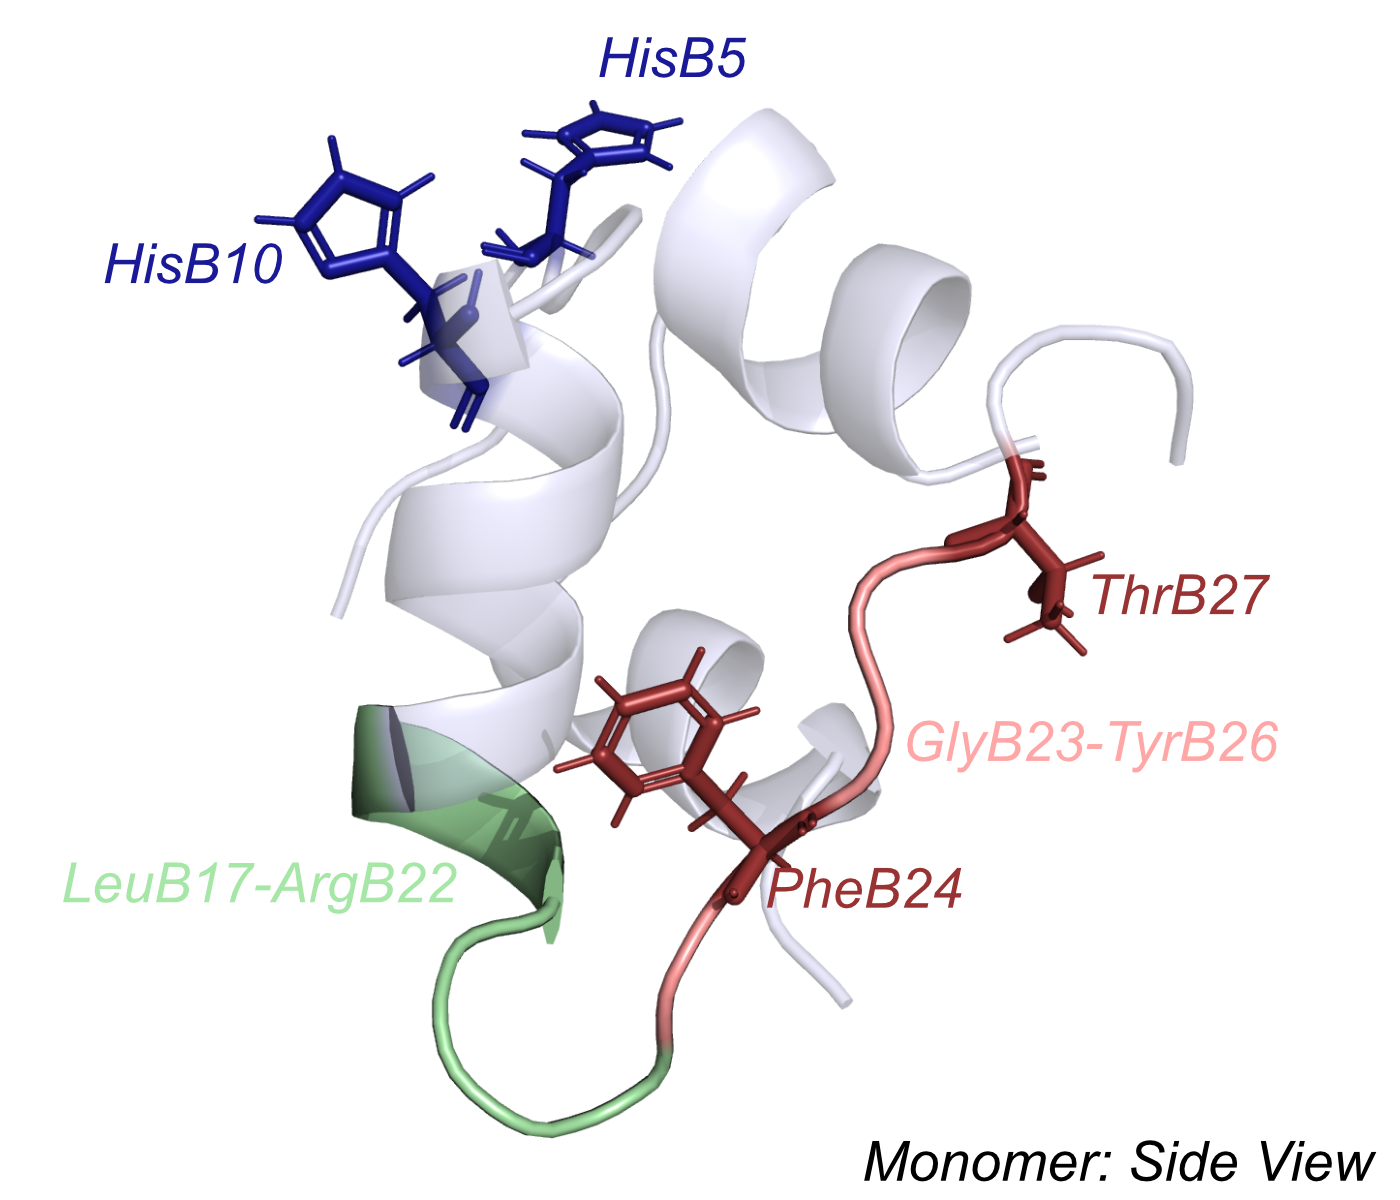
\includegraphics[width=0.6\textwidth]{Figures/Fig_histidine_WT.png}
\caption{The histidine residues (HisB5, and HisB10, colored in blue) are shown with residues PheB24 and ThrB27 (colored red) which are important in enhancing proteolytic stability and residues LeuB17-ArgB22 (colored green) and GlyB23-TyrB26 (colored salmon), important in determining dimerization potential.}
\label{supple_fig: WT_hist}
\end{figure}

\renewcommand{\thefigure}{S\arabic{figure}}
\begin{figure}[H]
\centering
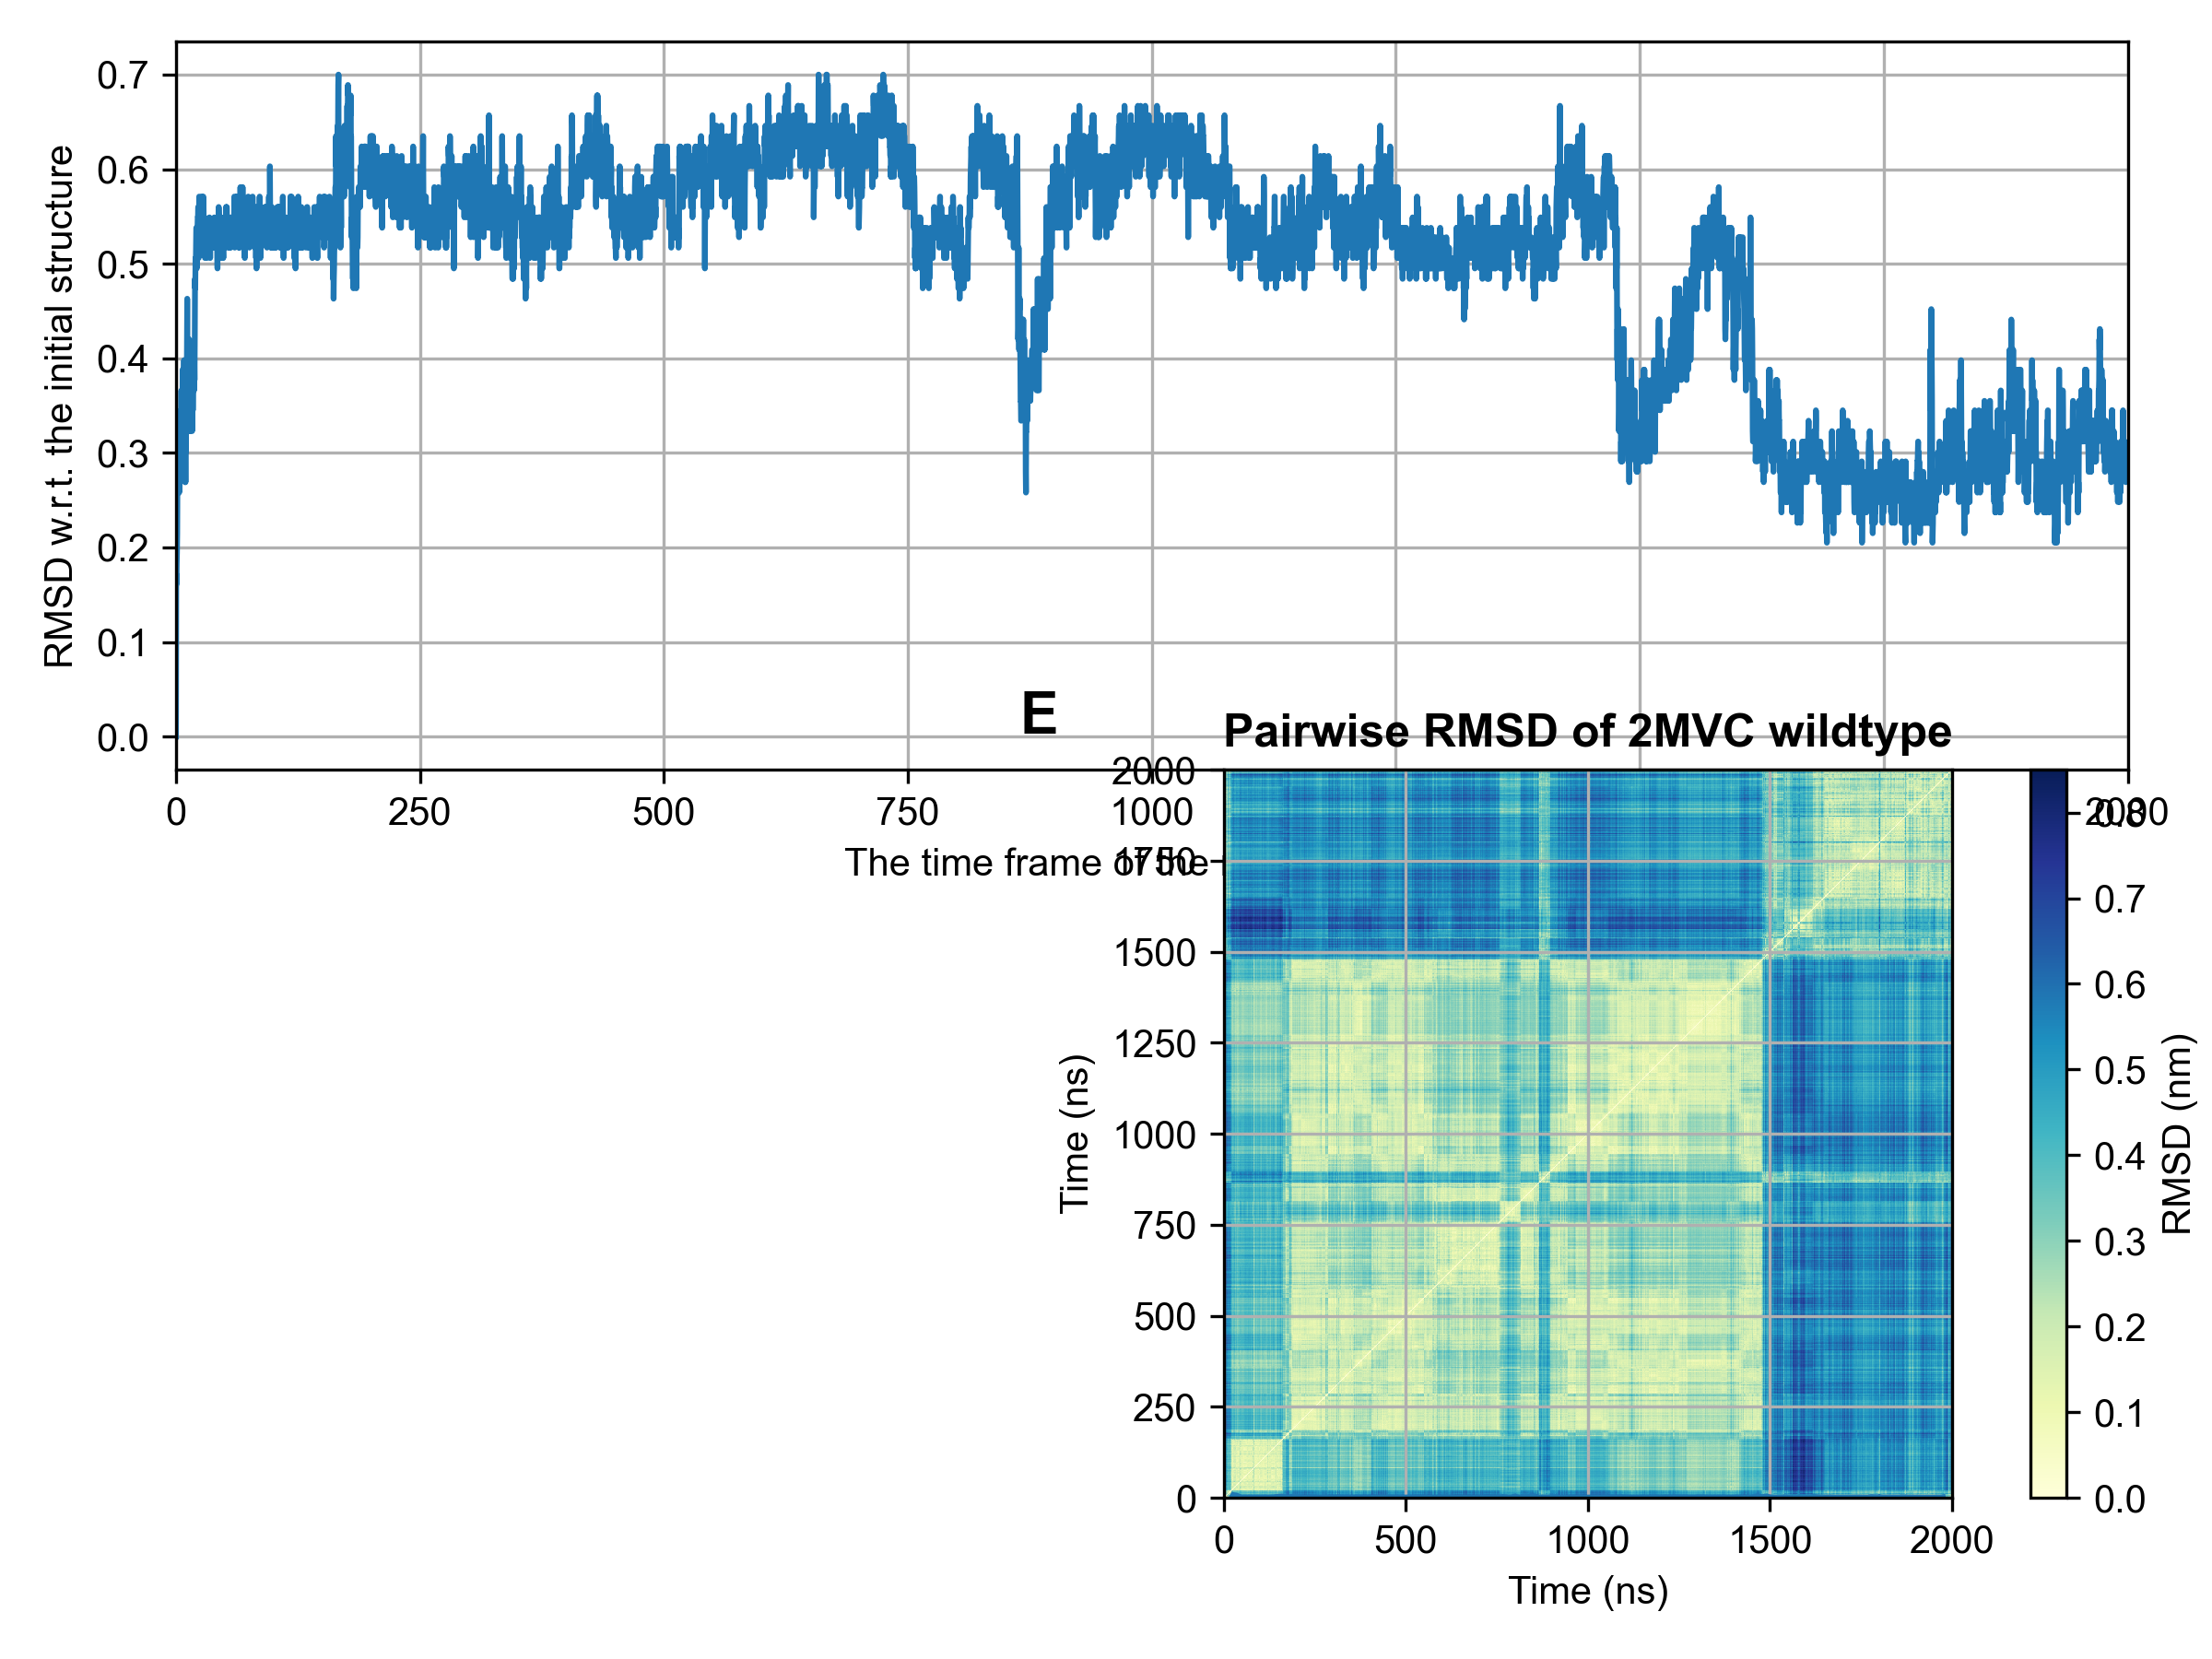
\includegraphics[width=\textwidth]{Figures/all_pairwise_rmsd.png}
\caption{The pairwise RMSD of calculated from the 250ps-spaced MD trajectory of each wild-type model, including 4EYD (A), 4EY9 (B), 4EY1 (C), 3I3Z (D), and 2MVC (E). As shown in the figure, the major transitions occur around 500--1500 ns, we therefore concluded that at least 2000 ns was required to sample the configurational ensemble of insulin.}
\label{supple_fig: pairwise_rmsd}
\end{figure}



\renewcommand{\thefigure}{S\arabic{figure}}
\begin{figure}[H]
\centering
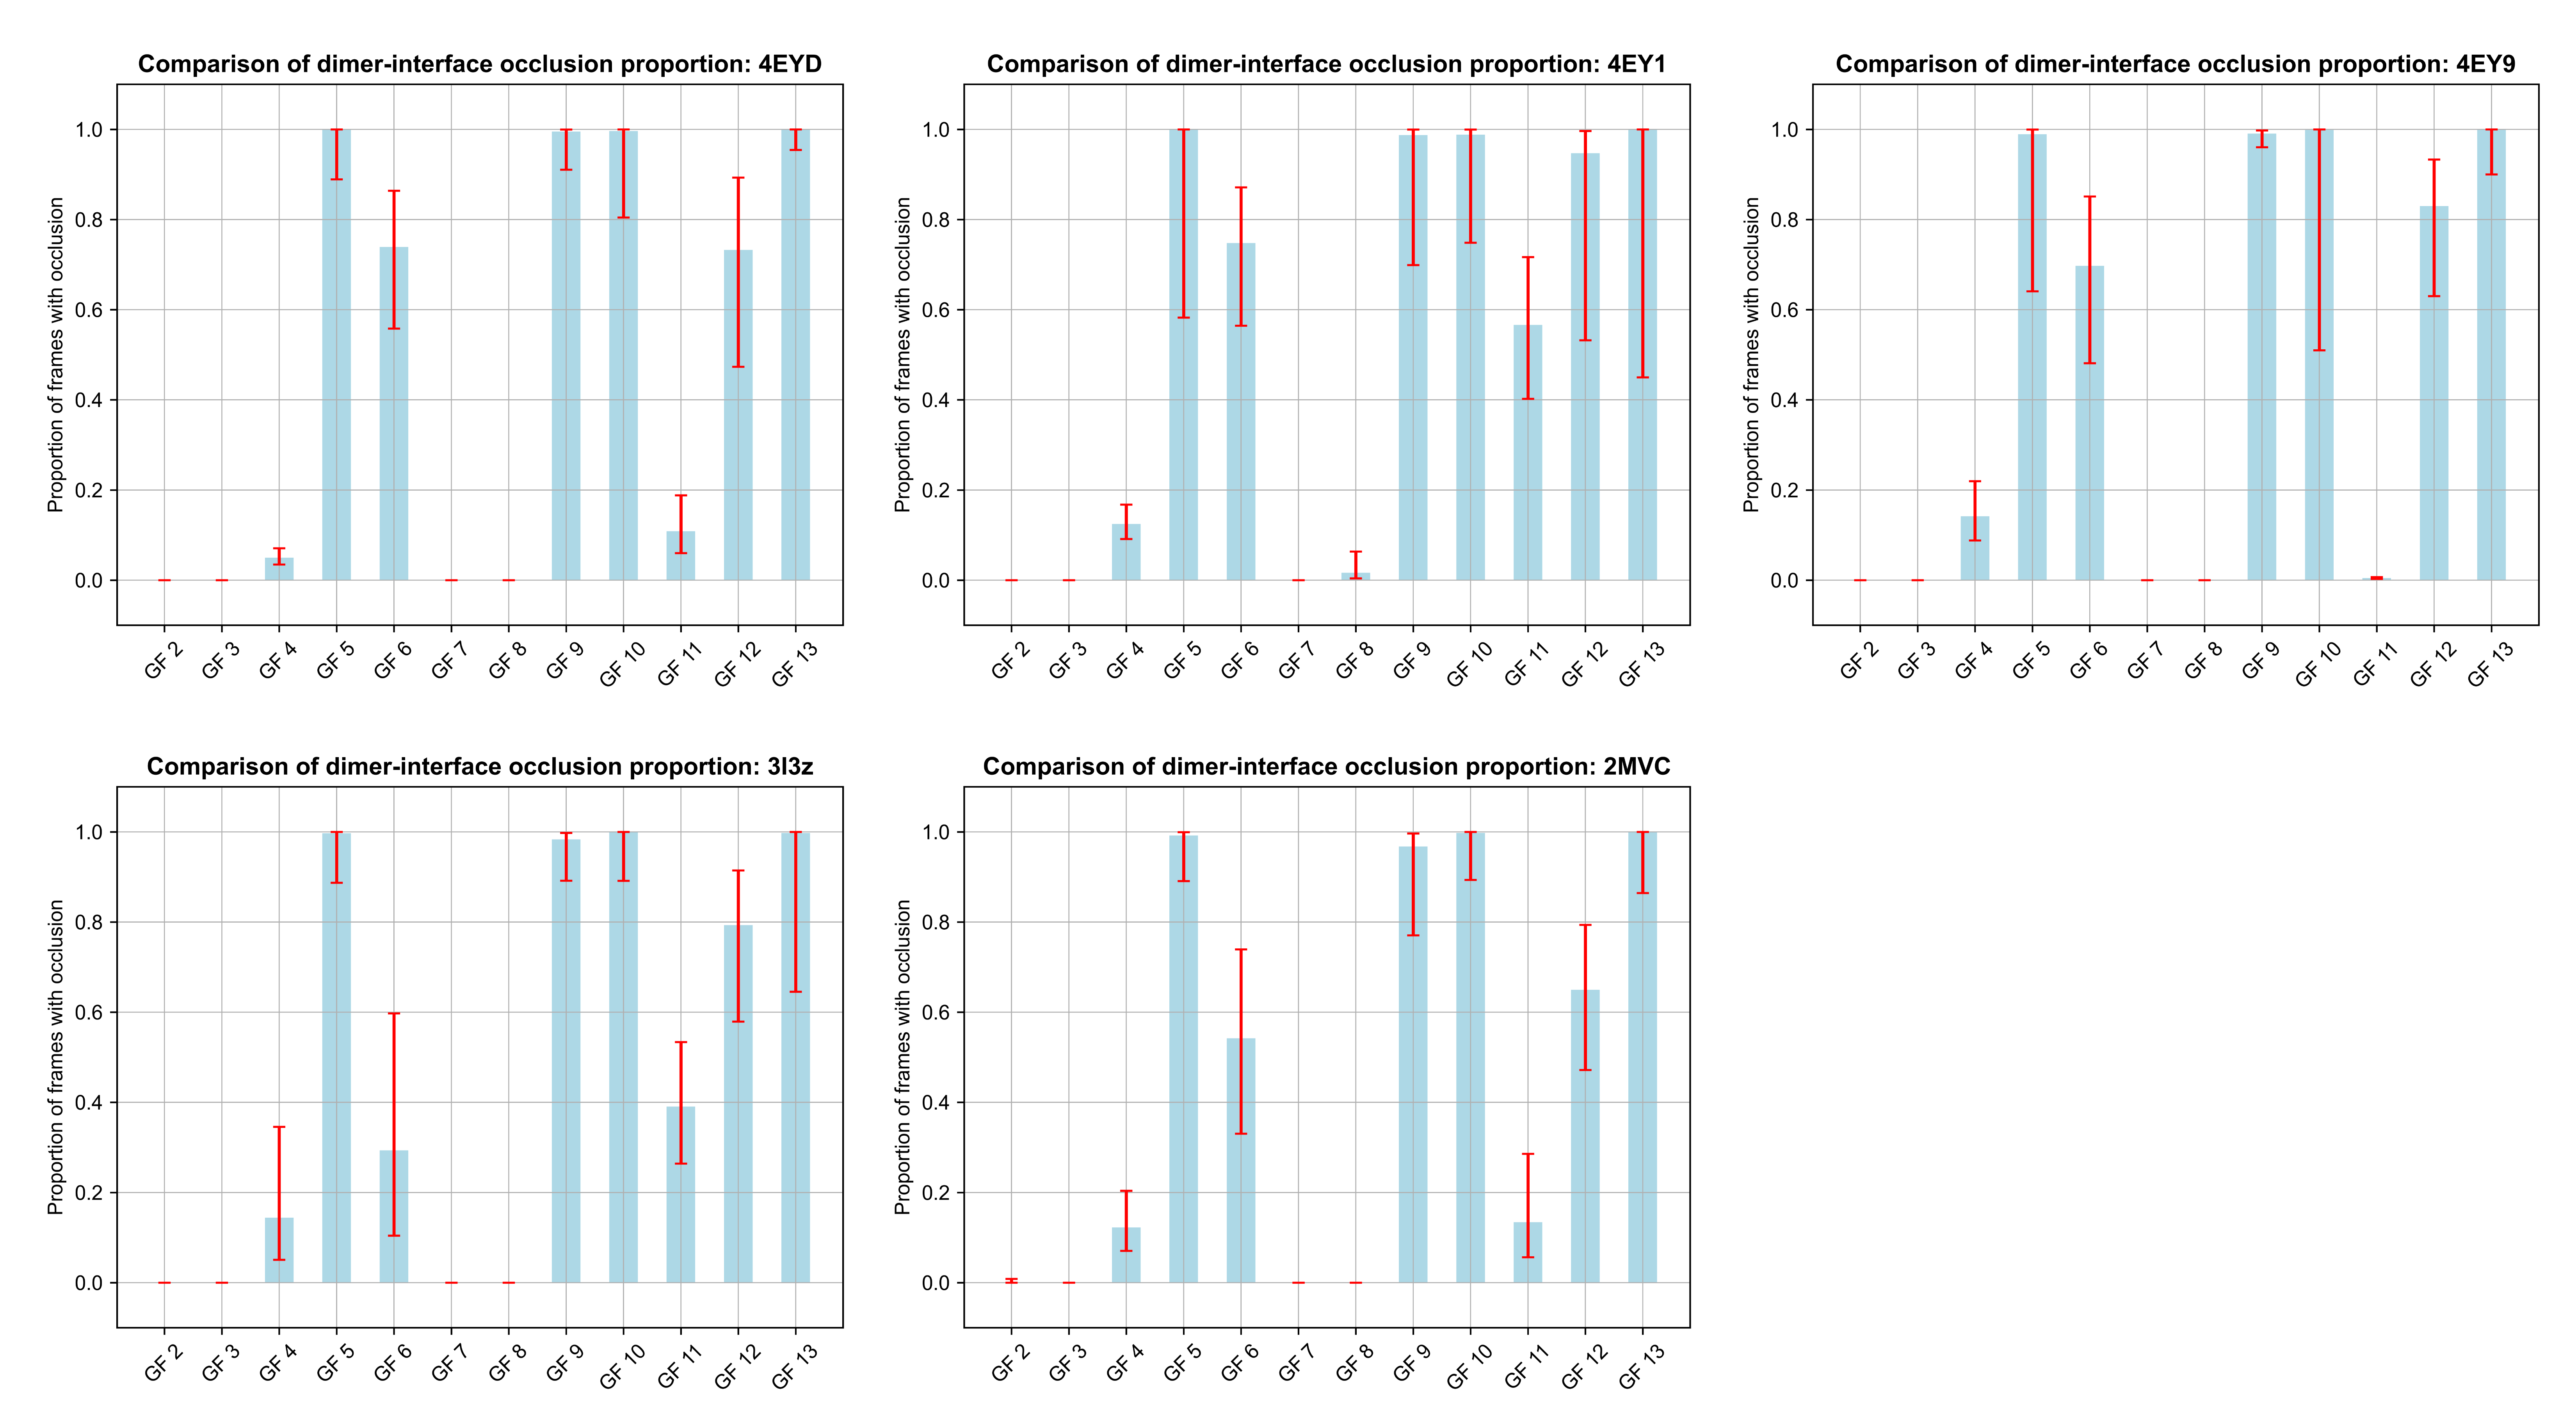
\includegraphics[width=1.0\textwidth]{Figures/occlusion_proportion_models_2.png}
\caption{Proportion of frames with glycan-dimer occlusion for each glycoform. Red bars represent the asymmetric 95\% Wilson score confidence interval.}
\label{supple_fig: occlusion_binomial}
\end{figure}

\end{document}
